\section{Теоретические основы расчёта электрических цепей постоянного тока}

\subsection{Основные законы электротехники}

Расчёт любой электрической цепи базируется на фундаментальных законах.

Закон Ома для участка цепи устанавливает связь между током \(I\), напряжением \(U\) и сопротивлением \(R\):

\begin{equation}
I = \frac{U}{R} \label{eq:ohm}
\end{equation}

где:
\begin{itemize}
    \item \(I\) --- сила тока, А;
    \item \(U\) --- напряжение, В;
    \item \(R\) --- электрическое сопротивление, Ом.
\end{itemize}

Из закона Ома также следуют производные формы:
\begin{equation}
U = I \cdot R, \quad R = \frac{U}{I} \label{eq:ohm2}
\end{equation}

Первый закон Кирхгофа (правило узлов): алгебраическая сумма токов в любом узле электрической цепи равна нулю:

\begin{equation}
\sum_{k=1}^{n} I_k = 0 \quad \text{или} \quad \sum I_{\text{вх}} = \sum I_{\text{вых}} \label{eq:kirchhoff1}
\end{equation}

Второй закон Кирхгофа (правило контуров): в любом замкнутом контуре алгебраическая сумма падений напряжений равна алгебраической сумме ЭДС:

\begin{equation}
\sum_{k=1}^{n} U_k = \sum_{m=1}^{m} E_m \label{eq:kirchhoff2}
\end{equation}

Мощность в электрической цепи --- физическая величина, характеризующая скорость передачи электрической энергии:

\begin{equation}
P = U \cdot I = I^2 \cdot R = \frac{U^2}{R} \label{eq:power}
\end{equation}

\subsection{Расчётная схема и математическая модель}

Рассматривается электрическая цепь постоянного тока со смешанным соединением резисторов рис. \ref {img:pic1}. Схема включает один источник напряжения \(U\) и три резистора \(R_1\), \(R_2\), \(R_3\), соединённых следующим образом: резистор \(R_1\) включён последовательно, а резисторы \(R_2\) и \(R_3\) соединены параллельно.

\begin{figure}[H]
    \centering
    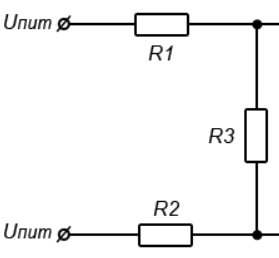
\includegraphics[scale = 0.8]{pic1.png}
    \caption{Электрическая цепь постоянного тока}
    \label{img:pic1}
\end{figure} 

\subsection{Пример ручного расчёта}

Выполним ручной расчёт для следующих исходных данных:
\begin{itemize}
    \item \(U = 100\) В
    \item \(R_1 = 100\) Ом
    \item \(R_2 = 200\) Ом
    \item \(R_3 = 300\) Ом
\end{itemize}

Результаты расчёта сведены в Таблицу 1.

\begin{table}[H]
    \centering
    \caption{Результаты ручного расчёта параметров цепи}
    \begin{tabular}{|c|c|c|c|}
        \hline
        \textbf{Параметр} & \textbf{Обозначение} & \textbf{Значение} & \textbf{Ед. изм.} \\
        \hline
        Эквивалентное сопротивление R2 и R3 & \(R_{23}\) & 120,00 & Ом \\
        Общее сопротивление цепи & \(R_{\text{общ}}\) & 220,00 & Ом \\
        Общий ток цепи & \(I_{\text{общ}}\) & 0,4545 & А \\
        Ток через резистор R1 & \(I_1\) & 0,4545 & А \\
        Ток через резистор R2 & \(I_2\) & 0,2727 & А \\
        Ток через резистор R3 & \(I_3\) & 0,1818 & А \\
        Напряжение на резисторе R1 & \(U_1\) & 45,45 & В \\
        Напряжение на участке R2-R3 & \(U_{23}\) & 54,55 & В \\
        Мощность на резисторе R1 & \(P_1\) & 20,66 & Вт \\
        Мощность на резисторе R2 & \(P_2\) & 14,88 & Вт \\
        Мощность на резисторе R3 & \(P_3\) & 9,92 & Вт \\
        Мощность источника & \(P_{\text{ист}}\) & 45,45 & Вт \\
        Суммарная мощность нагрузки & \(P_{\text{нагр}}\) & 45,46 & Вт \\
        Погрешность баланса & \(\delta\) & 0,02 & \% \\
        \hline
    \end{tabular}
    \label{tab:manual}
\end{table}